\documentclass[letter,11pt]{article}

\usepackage[spanish,es-nodecimaldot]{babel}
\usepackage[utf8]{inputenc}

\usepackage{lmodern}
\usepackage[T1]{fontenc}
\usepackage{textcomp}

\usepackage{framed}
\usepackage[svgnames]{xcolor}
\colorlet{shadecolor}{Gainsboro!50}

\usepackage{graphicx}
\usepackage{pstricks}

\usepackage{anysize}
\marginsize{3cm}{2cm}{2cm}{3cm}

\usepackage{siunitx}
\usepackage{amsmath}
\usepackage{array}

\usepackage{fancyhdr}
\usepackage{lastpage}
\pagestyle{fancy}
\fancyhf{}
\fancyhead[LE,RO]{Física Básica III}
\fancyfoot[CO,CE]{\thepage\ de \pageref{LastPage}}

\special{papersize=215.9mm,279.4mm}

\usepackage[
    pdfauthor={Carlos Eduardo Caballero Burgoa},%
    pdftitle={Física Básica III},%
    pdfsubject={1er Parcial},%
    colorlinks,%
    citecolor=black,%
    filecolor=black,%
    linkcolor=black,%
    urlcolor=black,
    breaklinks]{hyperref}
\usepackage{breakurl}

\newcommand{\blankpage}{
\newpage
\thispagestyle{empty}
\mbox{}
\newpage
}

\renewcommand{\arraystretch}{1.2}

\begin{document}

\begin{center}
    {\Large \bf{Primer parcial}}
\end{center}

\noindent\fbox{%
    \parbox{\textwidth}{%
        Estudiante: CABALLERO BURGOA, Carlos Eduardo \\
        Carrera: Ingeniería Electromecánica \\
        Correo: cijkb.j@gmail.com
    }%
}

\vspace{0.5cm}

\begin{enumerate}
\item Una varilla delgada de longitud $2L$ ($L = 1 [m]$) y uniformemente cargada
por unidad de longitud ($\lambda = 1 [\mu C/m]$), yace a lo largo del eje $x$,
como se muestra en la figura. Calcular el campo eléctrico en el punto $P$, a una
distancia $d = 1 [m]$ de la varilla a lo largo de su bisectriz perpendicular.

\begin{figure}[!h]
\centering

\includegraphics[scale=1.60]{resources/q1.eps}
\end{figure}

\begin{itemize}
    \item \textcolor{red}{$12727.92 [N/C]$.}
    \item $11462.36 [N/C]$.
    \item $10354.28 [N/C]$.
    \item $ 9658.33 [N/C]$.
\end{itemize}

\textbf{Solución:} \\

\begin{figure}[!h]
\centering
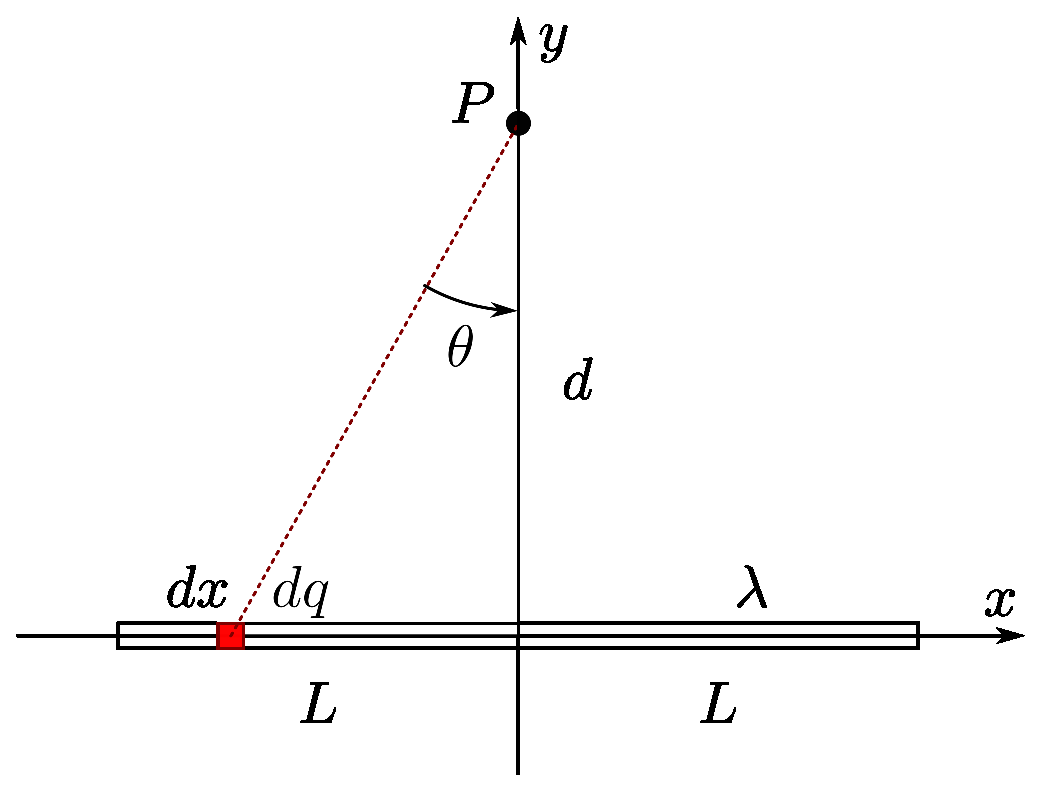
\includegraphics[scale=0.39]{resources/a1.eps}
\end{figure}

Dada la ecuación campo electrico:

\begin{equation*}
    \vec{E} = \frac{1}{4\pi\epsilon_0}\int_{Q}\frac{dq}{\vec{r}^2}
\end{equation*}

Y considerando la uniformidad de la carga:

\begin{equation*}
    \lambda = \frac{dq}{dx}
\end{equation*}

Entonces:

\begin{equation*}
    E_x = \frac{1}{4\pi\epsilon_0}\int_{-L}^{L}\frac{\lambda dx}{x^2+d^2}\,sen(\theta) = \frac{\lambda}{4\pi\epsilon_0}\int_{-L}^{L}\frac{dx}{x^2+d^2}\frac{x}{\sqrt{x^2+d^2}}
\end{equation*}
\begin{equation*}
    E_x = \frac{\lambda}{4\pi\epsilon_0}\int_{-L}^{L}\frac{x}{(x^2+d^2)^{3/2}}dx = \frac{\lambda}{4\pi\epsilon_0}\left(-\frac{1}{\sqrt{x^2+d^2}}\Biggr|_{-L}^{L}\right) = 0
\end{equation*}
\begin{equation*}
    E_y = \frac{1}{4\pi\epsilon_0}\int_{-L}^{L}\frac{\lambda dx}{x^2+d^2}\,cos(\theta) = \frac{\lambda}{4\pi\epsilon_0}\int_{-L}^{L}\frac{dx}{x^2+d^2}\frac{d}{\sqrt{x^2+d^2}}
\end{equation*}
\begin{equation*}
    E_y = \frac{\lambda\,d}{4\pi\epsilon_0}\int_{-L}^{L}\frac{1}{(x^2+d^2)^{3/2}}dx = \frac{\lambda}{4\pi\epsilon_0}\left(\frac{1}{d^2}\frac{x}{\sqrt{x^2+d^2}}\Biggr|_{-L}^{L}\right)
\end{equation*}
\begin{equation*}
    E_y = \frac{\lambda}{4\pi\epsilon_0}\left(\frac{2}{d^2}\frac{L}{\sqrt{L^2+d^2}}\right) = \frac{1}{4\pi\epsilon_0}\frac{2L\lambda}{d^2\sqrt{L^2+d^2}} = 12710.32 [N/C]
\end{equation*}

\item Considere un cilindro hueco con una pared delgada uniformemente cargada
con una carga total $Q = 1 [\mu C]$, radio $R = 0.1 [m]$ y una longitud
$L = 1 [m]$. Determine el campo eléctrico en un punto del eje a una distancia
$d = 0.2 [m]$ del lado derecho del cilindro como se muestra en la figura.

\begin{figure}[!h]
\centering

\includegraphics[scale=1.80]{resources/q2.eps}
\end{figure}

\begin{itemize}
    \item $41326.35 [N/C]$.
    \item $32775.13 [N/C]$.
    \item $25689.22 [N/C]$.
    \item $18567.46 [N/C]$.
\end{itemize}

\textbf{Solución:} \\

\item  Un cilindro aislante de longitud infinita y de radio $R = 0.3 [m]$, tiene
una densidad de carga volumétrica $\rho = \rho_0 (a - r/b )$ que varía en función del
radio donde $A_0 = 1 [\mu C/m^3]$, $a = 4$, y $b = 2$ son constantes positivas y
$r$ es la distancia al eje del cilindro. Calcule la magnitud del campo eléctrico
en $r = 1 [m]$.

\begin{itemize}
    \item $19830.51 [N/C]$.
    \item $18575.46 [N/C]$.
    \item $17624.33 [N/C]$.
    \item $16458.29 [N/C]$.
\end{itemize}

\textbf{Solución:} \\

\item Un alambre con una densidad lineal de carga uniforme igual a
$1 [\mu C/m]$, se dobla como se muestra en la figura. Calcular el potencial
eléctrico en el punto $0$.

\begin{figure}[!h]
\centering

\includegraphics[scale=1.80]{resources/q4.eps}
\end{figure}

\begin{itemize}
    \item $43419.92 [V]$.
    \item $44603.85 [V]$.
    \item $46371.26 [V]$.
    \item $48049.36 [V]$.
\end{itemize}

\textbf{Solución:} \\

\item Un capacitor de placas paralelas de $2 [nF]$ se carga con una diferencia
de potencial de $100 [V]$ y se aísla (desconecta de la batería) a continuación.
El material dieléctrico que llevaba entre las placas es mica con una constante
dieléctrica de $5$. Calcular el trabajo que se requiere para retirar la hoja de
mica.

\begin{itemize}
    \item $38 [\mu J]$.
    \item $39 [\mu J]$.
    \item $40 [\mu J]$.
    \item $41 [\mu J]$.
\end{itemize}

\textbf{Solución:} \\

\end{enumerate}

\end{document}

